\section{Програмна реалізація}
В якості мови програмування було обрано Python, оскільки це високорівнева інтерпретована мова програмування, що дозволяє швидко здійснювати побудову прототипу та скорочує час на розробку продукту вцілому. Значна частина системи являє собою веб-додаток, що стало ще одним фактором під час вибору даної мови, оскільки вона є веб-орієнтованою та містить величезну кількість бібліотек та сторонніх модулів для розробки саме веб-ресурсів. Python також дуже часто використовують в сфері збору та аналізу даних, тому що за рахунок можливості роботи в інтерактивному режимі інтерпретатора можливо значно зекономити час під час роботи з будь-якого роду даними. Гомогенність мов розроблюваних додатків дозволяє зберігати контекст і не перемикатися на синтаксичні відмінності чи особливості мови під час розробки програми. Це, в свою чергу, зменшує час на написання та дозволяє уникнути необхідності працювати з декількома різними мовами одночасно.
\textit{aiohttp} був обраний в якості веб-фреймворку за рахунок своєї асинхронної природи: оскільки основна мета веб-ресурсу коректно обробити вхідні дані від усіх користувачів, потрібно мати змогу асинхронно опрацьовувати велику кількість з'єднань. \textit{Redis} було обрано в якості локальної бази даних за рахунок його швидкодії. Дані зберігаються не на диску, а в пам'яті, що доволяє значно прискорити швидкодію в ситуаціях постійної роботи з записом та читанням. \textit{Redis} також дозволяє здійснювати операцію зберігання поточного стану на диск, тому було також розроблено компонент, що виконує дану діяльність періодично протягом всього часу роботи системи.

\begin{figure}[h!]
  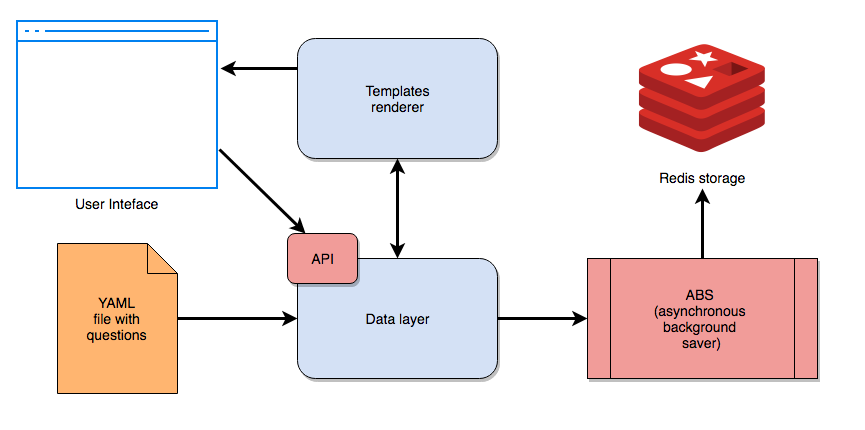
\includegraphics[width=\linewidth]{figures/poll_framework_architecture.png}
  \caption{Гістограма розподілу кількості клієнтів за віком}
  \label{fig:poll_framework_architecture}
\end{figure}

Архітектура мікросервісів була обрана значною мірою тому, що в даному програмному продукті ми маємо окремі повністю незалежні компоненти, які до того ж відповідають за зовсім різні функції системи. Виокремлення системи збору даних дозволяє як і розробляти її окремо та незалежно від інших складових, так і використовувати її в рамках інших систем, а зібрані в результаті її роботи дані в рамках будь-яких інших додатків. Платформа збору даних може бути використана взагалі незалежно в якості платформи для опитування, оскільки була розроблена як фреймворк і відповідно налаштовується під конкретні вимоги користувача. Архітектура фреймворку для опитування зображена на рис. \ref{fig:poll_framework_architecture}.

\subsection{Збір та попередня обробка даних}
Напрямок збору даних розвивався разом з розвитком комунікаційних технологій, а особливо як складова будь-якого бізнес процесу компаній. Проблеми оптимізації систем роботи з клієнтами спричинили появу підходів, які зараз вважаються класичними. В переважній більшості ці підходи покривають 99,9\% поточних бізнес задач. Враховуючи те, що за мету було поставлено не тільки розробку самого алгоритму для побудови моделі, але й збір даних для перевірки роботи цієї моделі, постала потреба загрегувати дані, представити їх у необхідному форматі та обробити їх належним чином. Для роботи з даними була обрана бібліотека \textit{Pandas}, а для роботи безпосередньо з числовими даними, векторами та статистичними функціями - бібліотека \textit{NumPy}. Серед науковців та спеціалістів з обробки даних також широко використовується мова програмування \textit{R}, яка уже містить значну частину вбудованих методів та навіть засобів візуалізації в стандарнтій бібліотеці самої мови, та \textit{Python} був обраний з урахуванням необхідності розробки всього програмного комплексу в рамках однієї мови програмування.

Процес обробки даних, трансформації значень та представлення даних в узагальненому форматі можна зобразити у вигляді діаграми на рис. \ref{fig:data_processing}

\begin{figure}[h!]
  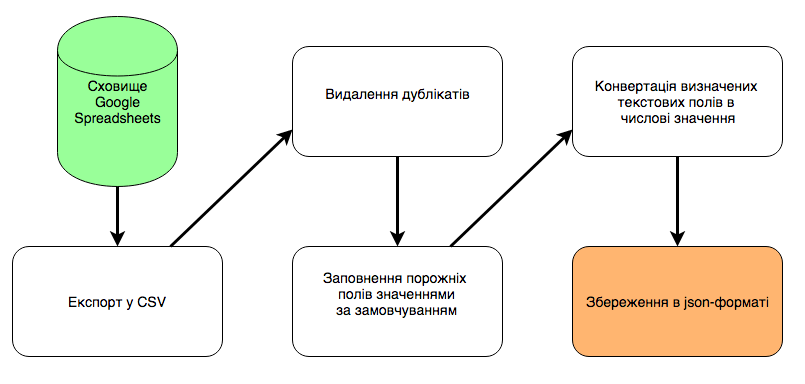
\includegraphics[width=\linewidth]{figures/data_processing.png}
  \caption{Етапи попередньої обробки даних}
  \label{fig:data_processing}
\end{figure}

В кінцевому результаті дані зберігаються в уніфікованому \textit{json}-форматі, що дає змогу: використовувати їх безпосередньо в консолі браузера для простішого перегляду і відлагодження; проводити легку конвертацію в \textit{csv}-формат, який очікує більшість інструментів з обробки даних; перетворювати їх в \textit{Python}-об'єкти для роботи з ними в коді програми; передавати на обробку в інші методи та функції, що вже готові працювати з даним форматом без необхідності додаткових серіалізацій/десеріалізацій; здійснювати конвертацію цих даних з додаванням відношень і зв'язків між ними (наприклад, для зберігання в реляційній \textit{SQL}-базі даних); зберігати на диск з можливістю перегляду в будь-якому текстовому редакторі.

Перед етапом обробки даних та жорсткого втручання в них (видалення записів, модифікація існуючих значень, заміна чи конвертація полів) необхідно мати загальне уявлення про вміст та загальні характеристики даних. На даному етапі на допомогу приходить статистика та її методи.
\textit{Статистика} - за своїм строгим визначенням не є технологією збору даних, проте саме вона використовується задля того, що знайти закономірності в даних та для наступної побудови прогностичних моделей. Також, з точки зору користувача, ви завжди будете стикатися з тими чи іншими інструментами статистики в будь-яких інших методах збору та аналізу даних. Статистика загалом являє собою розділ математики, пов'язаний зі збором та описом даних. Статистика займається підрахунком ключових значень та ймовірностей. Використання її в процесі збору даних допомагає відповісти на ряд важливих запитань, що відносяться до ваших даних: які закономірності прослідковуються з базі даних; яка ймовірність того, що обрана подія настане; які закономірності найбільш важливі; яку загальну інформацію можна отримати про дані, щоб зрозуміти з якого роду значеннями ми маємо справу.

Дану інформацію надалі можна використовувати для роботи з даними, оскільки це свого роду надає додаткову інформацію про доменну область (наприклад, на рис. зображена гістограма, що дає змогу швидко встановити факт про вік переважної кількості цільової аудиторії: більше 50). Інші з найчастіше вживаних метрик статистики:
\begin{itemize}
	\item \textit{max} - максимальне значення цільової величини;
	\item \textit{min} - мінімальне значення цільової величини;
	\item \textit{mean} - середнє значення обраної величини;
	\item \textit{median} - значення, що розділяє вибірку на дві підмножини з максимально наближеної кількістю елементів у кожній;
	\item \textit{mode} - значення, що зустрічається найчастіше;
	\item \textit{variance} - показник відхилення цільового значення від середнього у вибірці.
\end{itemize}

\begin{figure}[h!]
  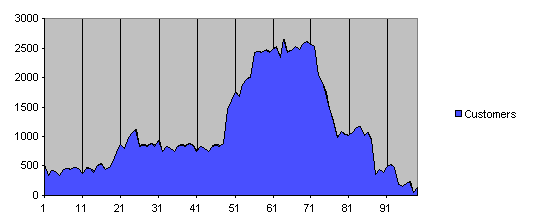
\includegraphics[width=\linewidth]{figures/statistics.png}
  \caption{Гістограма розподілу кількості клієнтів за віком}
  \label{fig:statistics}
\end{figure}

Останній показник, дисперсія, дещо складніший для розуміння: чим вище значення, тим більш дані різнорідні і різняться між собою. Якщо ж значення менше - дані загалом схожі і мало відрізняються від середнього по вибірці. Базуючись на статистичних даних, користувач має змогу налаштувати модель таким чином, щоб передбачуване значення максимально відоражало реальну зміну величини.

Для збору даних та формування початкового датасету було створено допоміжний додаток у вигляді веб-ресурсу. Він являє собою веб-сайт, на якому здійснюються опитування серед різних класів респондентів: студентів, випускників та викладачів. Кожен учасник опитування заповнює невелику тематичну анкету, на основі якої формуюється таблиця вхідних даних. Загальну архітектуру додатку можна побачити на рис. \ref{fig:poll_architecture} 

\begin{figure}[h!]
  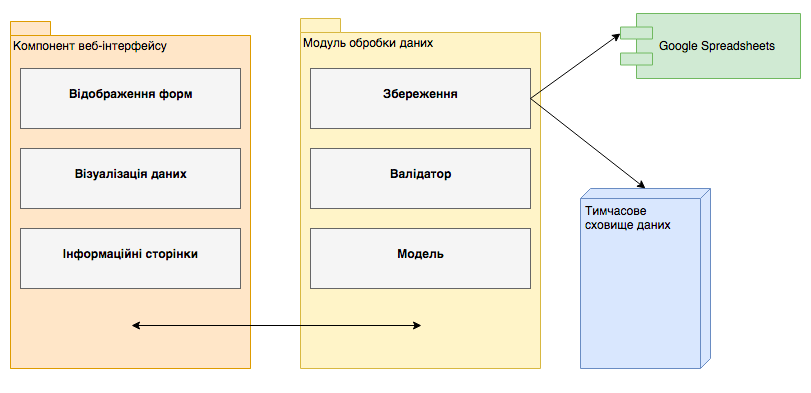
\includegraphics[width=\linewidth]{figures/poll_architecture.png}
  \caption{Загальна архітектура додатку опитування}
  \label{fig:poll_architecture}
\end{figure}

Система побудована на основі архітектури мікросервісів і дотримання принципу делегування частини роботи зовнішнім ресурсам. За рахунок такого підходу можна отримати більшу ефективність, стабільність та пропускну здатність роботи системи, але знижується надійність, оскільки вихід хоча б одного компоненту з ладу призведе до повної недієздатності системи. Враховуючи важливий фактор роботи з даними, потрібно розуміти, що втрати на етапі збору значно впливають на подальші результати. Саме тому було додамо внутрішнє тимчасове сховище даних, яке слугує для збереження резервних копій. Система складається з таких компонентів:
\begin{itemize}
	\item Веб-інтерфейс - являє собою веб-додаток, що побудований на основі aiohttp веб-фреймоврку та здійснює основні функції обробки користувацької логіки. Він відповідає за рендеринг сторінок, видачу статичних ресурсів, обробку та роутинг запитів та спілкується з іншими компонентами для подальшоої передачі даних. 
	\begin{itemize}
		\item Відображення форм - підкомпонент, що відповідає за відображення користувацького інтерфейсу та безпосередню взаємодію з користувачем за допомогою веб-браузера.
		\item Візуалізація даних - представлення вхідних, існуючих, а також відображення статусу обробки поточних даних для розуміння стану даних та прогресу під час заповнення форми опитування.
		\item Інформаційні сторінки - відображення статичних сторінок веб-ресурсу для надання додаткової інформації та для отримання зворотного зв'язку.
	\end{itemize}
	\item Модуль обробки даних - здійснює фільтрацію, нормалізацію та перетворення даних таким чином, щоб вони були уніфікованого формату та могли бути використанні надалі іншими компонентами. Обробка здійснюється з використанням можливостей самої мови, а також з допомогою сторонніх бібліотек \textit{NumPy} та \textit{Pandas}.
	\begin{itemize}
		\item Підкомпонент збереження даних - створення об'єктів для кінцевих даних форм на основі моделей; створення асинхронних задач збереження даних; переріодична інкрементальна відправка проміжного стану для формування єдиної бази, використовуючи сторонній сервіс \textit{Google Spreadsheets}. Збереження виконується як локально, використовуючи базу даних в оперативній пам'яті, так і віддалено, використовуючи основну базу даних на основі таблиць.
		\item Валідатор - здійснення перевірки даних на коректність та відповідність вхідним обмеженням. Видача повідомлень про помилку в разі невідповідності.
		\item Модель - \textit{data access object}, представлення вхідних даних у вигляді об'єктів мови програмування для надання зручного доступу до даних з коду програми. Серіалізація моделі дозволяє зберегти дані для подальшого використання та можливої додаткової обробки. За допомогою формального представлення даних у вигляді моделі можливо з легкістю проводити маніпуляції з даними в рамках інструментів мови програмування.
	\end{itemize}
\end{itemize}

Особливості даних можна встановити ще на етапі їх збору. Навіть не здійснюючи жодного аналізу чи попередньої обробки можливо отримати деякі важливі характеристики даних або просто візуалізувати їх для зручнішого сприйняття чи для кращого усвідомлення того, з якого роду даними доведеться працювати. Саме для таких цілей і використовується \textit{exploratory data analysis} - аналіз даних з метою попереднього дослідження вхідних даних.

Візуалізація даних загалом здійснюється для таких цілей:
\begin{itemize}  
	\item Комунікативна складова:
	\begin{itemize}
		\item представити дані та ідеї;
		\item проінформувати;
		\item підтримати і аргументувати;
		\item вплинути і переконати;
	\end{itemize}
	\item Дослідницька:
	\begin{itemize}
		\item вивчити (дослідити) дані;
		\item проаналізувати ситуацію;
		\item визначити наступні кроки;
		\item прийняти рішення стосовно деякого питання;
	\end{itemize}
\end{itemize}

Оскільки одним із компонентів збору даних був \text{Google Spreadsheets}, то початкова візуалізація даних не становила жодної складності, тому що даний ресурс містить вбудовані засоби для цього рис. \ref{fig:answer_visualize} 

\begin{figure}[h!]
  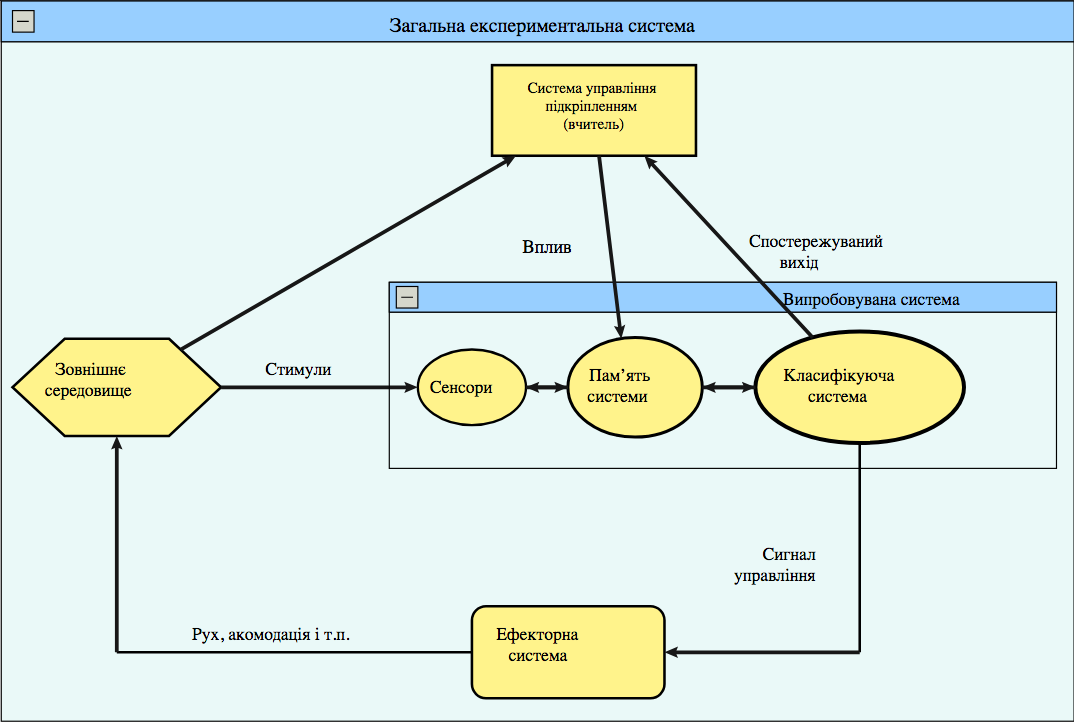
\includegraphics[width=\linewidth]{figures/fig_system.png}
  \caption{Візуалізація відповідей однієї з форм анкети опитування}
  \label{fig:answer_visualize}
\end{figure}

Для збору даних потрібно враховувати декілька важливих нюансів. По-перше, це \textit{робота з неповними даними} - ситуація, коли зібрані дані не віповідають поставленим критеріям чи не проходять валідацію, але не можуть бути відкинуті, оскільки є досить важливими. Схожа ситуація може відбутися, коли дані взагалі зберігаються в різної кількості форматах та структур, тому виділити один загальний критерій для валідації може бути досить важко. Тому потрібно завжди враховувати випадок обробки та роботи з неповними даними. 

\textit{Врахування ефективності алгоритмів, що використовуютьс з роботи з даними} - під час обробки невеликої кількості даних ефективність алгоритму не відіграє значної ролі, оскільки обчислювальних ресурсів комп'ютера зазвичай більш ніж досить, тому користувач майже не помічає затримок у роботі. Але з ростом об'єму даних (які можуть сягати декількох сот гігабайт) час на їх обробку може зростати нелінійно, а отже операції можуть перевищувати встановлені обмеження на тривалість роботи. Тому необхідно враховувати кількість даних, з якими повинна буде працювати системи і обирати максимально ефективні алгоритми для роботи.

\textit{Отримання великого обсягу початкових даних} - під час скрапінгу веб-ресурсів або під час потокового отримання вхідних даних (\textit{streaming}) можуть виникнути проблеми, пов'язані з неможливістю процесу обробити всі дані одночасно чи зберігати їх в рамках однієї сесії в оперативній пам'яті. Для вирішення такої проблеми можна скористатися такими підходами: кешування інформації на проміжних етапах, використання вбудованих функцій замість написання власних послідовностей обробки на стороні бізнес-логіки (прикладом може бути використання stored procedures під час роботи з \textit{SQL} базами даних), побудова алгоритмів, що використовують принцип \textit{pipeline} (вихід одніє функції відразу слугує вхідними даними для іншої, таким чином відпадає необхідність зберігати дані в проміжному стані та витрачати додатковий простір на жорсткому диску), пакетна обробка даних.

\textit{Обробка даних, що містять зв'язки між собою} - досить поширена ситуація, коли одні дані містять посилання на інші, або потрібно відслідковувати зв'язки між певними компонентами вхідної інформації. В такому випадку немає простих рішень чи рекомендації, оскільки в будь-якому випадку потрібно буде підтримувати структуру даних, що буде відповідати за збереження даних зв'язків. Очевидним рішенням є використання реляційних баз даних, які будуть підтримувати структуру і відношення чи альтернативне використання графових баз даних, принцип яких саме в побудові бази таким чином, щоб вона представляла собою граф відносин між даними.

\textit{Обробка даних, що містять зв'язки між собою} - досить поширена ситуація, коли одні дані містять посилання на інші, або потрібно відслідковувати зв'язки між певними компонентами вхідної інформації. В такому випадку немає простих рішень чи рекомендації, оскільки в будь-якому випадку потрібно буде підтримувати структуру даних, що буде відповідати за збереження даних зв'язків. Очевидним рішенням є використання реляційних баз даних, які будуть підтримувати структуру і відношення чи альтернативне використання графових баз даних, принцип яких саме в побудові бази таким чином, щоб вона представляла собою граф відносин між даними.

\textit{Підтримка гетерогенності джерел інформації} - системи, що використовуються для отримання даних можуть не мати уніфікованого інтерфейсу та не надавати однакові можливості зі свого боку для здійснення запитів. Потрібно враховувати відмінності між кожним окремим джерелом, а також розуміти встановлені обмеження (наприклад, багато веб-ресурсів встановлюють обмеження на кількість запитів, що здійснюються за певний проміжок часу). Тому якщо додаток буде розроблено без урахування таких відмінностей - він може показати добрі результати під час роботи з одним провайдером інформації, але для інших він не буде функціонувати належним чином.


\subsection{Побудова моделі}
Для створення ефективної кінцевої моделі розроблюваний алгоритм повинен підповідати таким вимогам:
\begin{itemize}  
	\item відкритий доступ користувача до коду моделі на будь-якій платформонезалежній мові, що дозволить запускати її в довільному середовищі та не опиратися на використання сторонніх бібліотек;
	\item будова моделі та деталі її внутрішньої реалізації повинні бути відкритими, тобто користувач повинен мати змогу переглянути вихідний код і в разі необхідності самостійно відтворити довільний крок та отримати аналогічний результат передбачення для однакового набору вхідних даних;
	\item модель повинна мати точність максимально наближену до точності моделей, що показують найкращі результати для вибраних вхідних даних. Модель повинна мати аналогічні показники щонайменше для 95\% всіх вхідних наборів даних;
	\item виконання коду програми повинно бути швидким (близько 1 мс на рядок вхідних даних).
\end{itemize}

Використовуючи отримані на попередніх етапах дані та проаналізувавши висунуті вимоги, опишемо розроблений алгоритм для побудови кінцевої моделі (припускаємо, що етап збору даних уже пройдено і вони зберігаються в централізованому сховищі):
\begin{enumerate}  
	\item Виконання алгоритмів попередньої обробки та трансформації даних для початкового "сирого" набору даних. Здійснюються всі необхідні кроки для очищення та нормалізації, а також побудова додаткової статистики для опису властивостей вхідних даних.
	\item Конвертація текстових даних для характеристичних змінних, що представлені не у числовому вигляді. На даному етапі здійснюється безпосереднє перетворення текстових даних в числовий чи векторний формат, з яким можуть працювати всі алгоритми класифікації.
	\item Визначення множини алгоритмів класифікації, для яких на основі вхідних даних буде відбуватися створення і тренування моделі. Наразі будуються всі моделі з множини наперед визначених алгоритмів не залежно від набору даних. Перед етапом побудови виконується поділ датасету на дані для тренування та валідації, а також допоміжні розділи, якщо цього вимагає алгоритм.
	\item Валідація всіх побудованих моделей та здійснення прогнозування досліджуваної величини. Також перевірка точності всіх моделей за обраною метрикою задля сортування та вибору найкращої з усіх моделей.
	\item Для обраної найкращої моделі виконати побудову "гібридної моделі" за допомогою методу \textit{RuleFit}, таким чином здійснити її апроксимацію для забезпечення мінімальної похибки передбачення, порівнюючи з базовою моделлю.
	\item Для всіх наступних даних, для яких ми хочемо прогнозувати значення досліджуваної величини, використовувати лише одну побудовану на попередньому етапі модель. Саме це забезпечить поєднання точності передбачення найкращої моделі та швидкодію реалізації кінцевої моделі.
	\item Здійснити збереження моделі для подальшого використання в разі надходження нових даних, якими ми хочемо скористатися для передбачення.
\end{enumerate}

Даний алгоритм можна спрощено зобразити у вигляді блок-схеми (рис. \ref{fig:alg_model}). Як бачимо на схемі, спочатку здійснюється побудова $N$ моделей, для кожної з яких проводиться тренування і методом оцінки за вибраним критерієм визначається найкраща з них. Потім на основі моделі, що дала найкращі показники, здійснюється побудова кінцевої "гібридної" моделі, що усюди надалі використовується для прогнозування передбачуваної величини.

\begin{figure}[h!]
  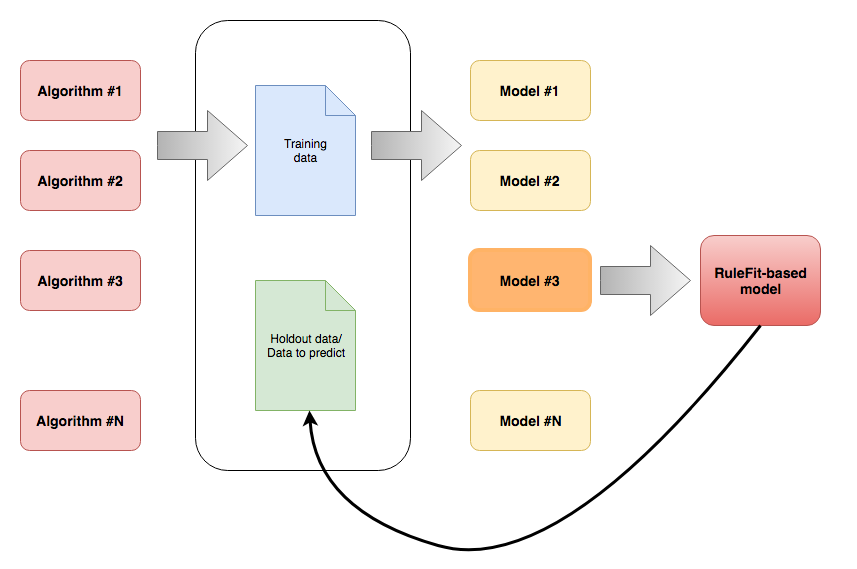
\includegraphics[width=\linewidth]{figures/alg_model.png}
  \caption{Алгоритм побудови гібридної моделі}
  \label{fig:alg_model}
\end{figure}

Можливий частковий випадок, коли декілька моделей будуть мати однакові показники для точності передбачення. В такому разі можна скористатися кількома метриками і оцінювати моделі за множиною параметрів, а не лише за одним критерієм. Також можливим рішенням є використання будь-якої моделі чи використання їх обох за умови, що витрати на час є доцільними. Одним із цікавих варіантів розвитку даного дослідження у такому випадку є створення деякої композиції $k$ найкращих моделей (використання їх паралельно та подальше усереднення результатів чи, в загальному випадку, створення деякої лінійної комбінації вихідних даних всіх моделей для подальшого визначення найбільш точного результату), що з точки зору інкапсуляцію будуть поводити себе як одна модель, проте давати більш точні передбачення, що безсумнівно є досить привабливою перевагою для науковців.

\subsection{Результати реалізації}
Отже, було розроблено три основних компоненти системи: програма-агрегатор у вигляді веб-додатку для накопичення та збереження сирих вхідних даних; програма для попередньої обробки, очищення та трансформації даних і, відповідно, збереження у форматі, готовому для роботи з алгоритмами класифікації; компонент, що здійснює побудову множини моделей, визначає найкращу з них та будує гібридну модель на її основі, а також безпосередньо використовується для подальшого прогнозування.

Реалізація стабільно показуює чудові результати валідації відносно базової моделі в межах допустимої похибки, а також аналогічні показники для даних, що прогнозуються. Задачі класифікації текстів дають дещо гірші показники за рахунок втрати даних на момент перетворення їх у числове представлення (для текстових категорій схожі втрати відстуні), але загалом не відрізнються від методів-аналогів. Головною підтвердженою перевагою залишається швидкодія робити в поєднанні зі збереженням допустимої точності моделі.